\section{Object Detection}
\label{sec:ObjectDetection}

Since the topic of this thesis concerns the task of \emph{visual} object tracking, an indispensable step in the processing pipeline will unquestionably be object detection. Holistically, there are \emph{fast} object detectors, such as the most prominent one, \gls{yolo}~\cite{redmon2016yolo} (\sectiontext{}~\ref{ssec:YouLookOnlyOnce}), or \gls{ssd}~\cite{liu2016ssd}. Here, we use the term \emph{fast} to denote that the detector can operate on high \gls{fps}. This comes at a cost of relatively lower accuracy, though, as compared to \emph{slower} but more accurate approaches based on \glspl{rpn}, such as various versions of \gls{fasterrcnn} (\sectiontext{}~\ref{ssec:FasterRCNN}).

Object detection is, by its very nature, a difficult task, because the number of objects is unknown in advance, which means, that the number of outputs of the model is variable. A plethora of attempts have been proposed to evade this inherent shortage of standard neural networks. An obvious solution is to only produce a constant number of \glspl{bbox}, as utilized by \gls{ssd} and \gls{yolo}, for instance. But methods based on \glspl{rpn} try to circumvent the obstacle of having to predict only a fixed set of \glspl{bbox}. Other differences between object detectors stem from the architecture itself, whether the training is an end-to-end pipeline or the model consists of various parts. Fully convolutional architectures are also becoming more prevalent~\cite{tian2019fcos}.

% ##############################################################################
\subsection{Non-Maximum Suppression}
\label{ssec:NonMaximumSuppression}

Object detectors have hugely profited from the end-to-end learning paradigm in which features, object proposals, and the classifier become part of one model~\cite{hosang2017learningnms}. A proposal is nothing but a region containing a potential object of interest. However, the number of proposals may grow considerably, outnumbering the real count of present objects. Moreover, these proposals may have a large overlapping region as measured by \gls{iou} (\sectiontext{}~\ref{eq:IntersectionOverUnion}), rendering most of them useless in terms of conveying new information. To filter such proposals, the \gls{nms} algorithm introduced below is used (\figtext{}~\ref{fig:NonMaximumSuppression}). The objective is to iteratively select only proposals the \gls{iou} of which is below a specific threshold.

Let $\mset{B} = \cbrackets{\vect{b}_1, \vect{b}_2, \dots, \vect{b}_n}$ be a set of $n$ region proposals described by $n$ \glspl{bbox}. Scores for each detection are contained in a set $\mset{S} = \cbrackets{s_1, s_2, \dots, s_n}$, where $s_i$ denotes a detection score for the $i$-th box, $\vect{b_i}$. Let $\lambda$, such that $0 \leq \lambda < 1$, denote the threshold for the maximum allowed portion of the overlap between regions. $\mset{B}_{nms}$ is the set of filtered proposal instances from the set $\mset{B}$ produced using \gls{nms} (\algtext{}~\ref{alg:NonMaximumSuppression}).

\begin{algorithm}[t]
    \caption{Non-Maximum Suppression}
    \label{alg:NonMaximumSuppression}
    \begin{algorithmic}[1]
        \Function{NMS}{$\mset{B}$, $\mset{S}$, $\lambda$}

        \State $\mset{B}_{nms}$ $\gets$ $\emptyset$
        \Comment{initialize the output (filtered) set of region proposals}

        \While {$\mset{B} \neq \emptyset$}
        \Comment{loop until all the proposals are processed}

        \State $m \gets \underset{i \in \cbrackets{1, 2, \dots, \msetsize{S}}}{\argmax{}} \mset{S}$
        \Comment{find an index of a proposal with the highest score}

        \State $\mset{B} \gets \mset{B} - \vect{b}_m$, $\mset{S} \gets \mset{S} - s_m$
        \Comment{remove the proposal}

        \State $\mset{B}_{nms} \gets \mset{B}_{nms} \cup \vect{b}_m$
        \Comment{save the proposal with the highest score}

        \For{$i \gets 1$ to $\msetsize{B}$}
        \Comment{iterate through remaining proposals}

        \If{\Call{iou}{$\vect{b}_m$, $\vect{b}_i$} $\geq \lambda$}
        \Comment{\gls{iou} (\eqtext{}~\ref{eq:IntersectionOverUnion}) exceeds the threshold}

        \State $\mset{B} \gets \mset{B} - \vect{b}_i$, $\mset{S} \gets \mset{S} - s_i$
        \Comment{remove the proposal}
        \EndIf
        \EndFor
        \EndWhile

        \State \Return $\mset{B}_{nms}$
        \EndFunction
    \end{algorithmic}
\end{algorithm}

% ------------------------------------------------------------------------------
\begin{figure}[t]
    \centerline{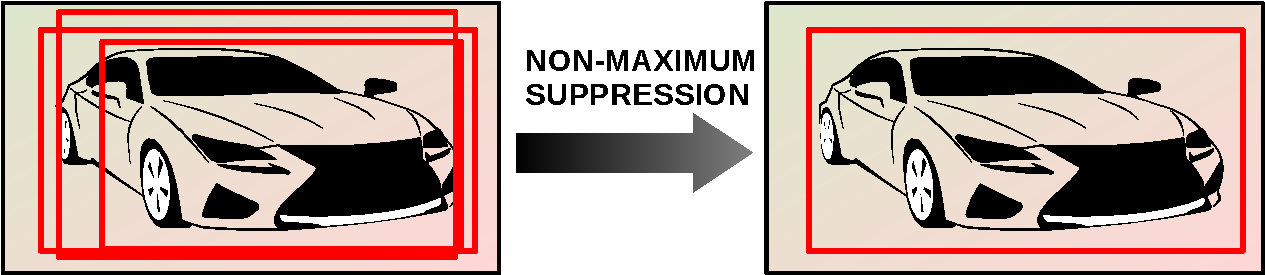
\includegraphics[width=0.6\linewidth]{figures/theoretical_foundations/non_maximum_suppression.pdf}}
    \caption[\Gls{nms} visualization]{An illustration of a potential effect of the \gls{nms} algorithm on \glspl{bbox}. Multiple proposals (left) are filtered so that only the ones with the highest detection score (right) remain while satisfying the condition that the overlap does not exceed a specific threshold.}
    \label{fig:NonMaximumSuppression}
\end{figure}
% ------------------------------------------------------------------------------

% ##############################################################################
\subsection{YOLO}
\label{ssec:YouLookOnlyOnce}

\Gls{yolo} is a very popular single-stage object detector thanks to its ability to run in real-time and yet be sufficiently accurate. Its speed is primarily a consequence that \emph{it looks only once} at a given input image. Compared to \gls{rpn}-based approaches, the authors of \gls{yolo} devised a \gls{cnn} model capable of performing extraction of region proposals as well as classification in a single run~\cite{redmon2016yolo}. Besides, the backbone \gls{cnn} model that is responsible for handling the visual input processes an entire image during the training and test time, allowing the implicit inclusion of contextual information about classes together with their visual representation. During the testing phase, after the single forward pass through the model, the \gls{nms} algorithm is employed to filter predictions to make sure that each object instance is detected just once. Since the initial introduction of this approach~\cite{redmon2016yolo}, multiple updates have been brought forward, either from the main author himself~\cite{redmon2017yolo9000, redmon2018yolov3} or from other researchers~\cite{wang2020yolov4, wong2019yolonano}. Despite its popularity, for our experiments, we employed the paragon of two-stage object detection, discussed next.

% ##############################################################################
\subsection{Faster R-CNN}
\label{ssec:FasterRCNN}

The \gls{fasterrcnn}~\cite{ren2017fasterrcnn} is the most prominent \emph{two-stage} object detector. The first stage consists of generating region proposals using the \gls{rpn}~\cite{huang2017speedacctradeoff}. These class-agnostic proposals, a set of rectangular \glspl{bbox}, are produced from an input of arbitrary size (allowed by the fact that this process is modeled by a fully convolutional network) (\figtext{}~\ref{fig:FasterRCNNPipeline}). As far as the second stage is concerned, the proposed regions (usually $300$) serve as a basis for subsequent cropping of features from the same intermediate feature maps that are then fed to the remaining feature extractor to predict the class. Based on this class prediction, the proposed box is further refined.

As the endeavor is to diminish unnecessary computations, the proposals are not cropped explicitly from the input image, and then processed by the feature extractor. Nevertheless, there is a part of the computation that has to be executed once per each proposed region, so the performance depends on the number of regions generated by the \gls{rpn}.

% ------------------------------------------------------------------------------
\begin{figure}[t]
    \centerline{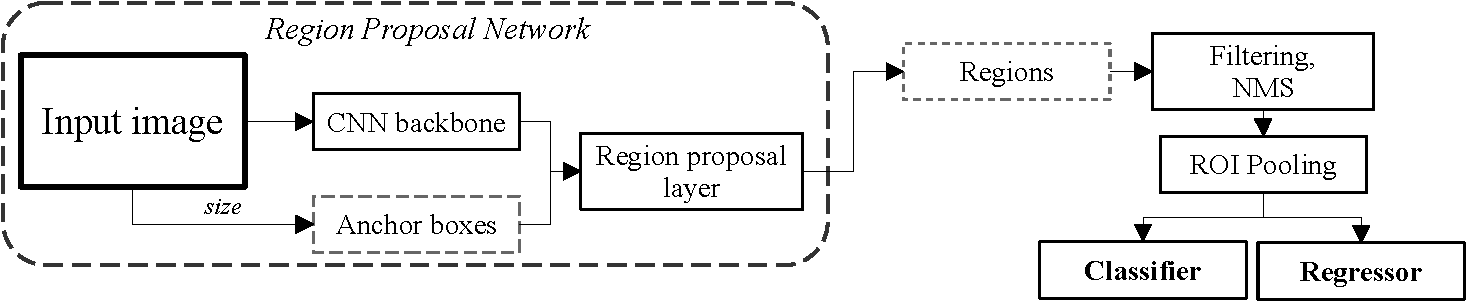
\includegraphics[width=\linewidth]{figures/theoretical_foundations/fastercnn_diagram.pdf}}
    \caption[\gls{fasterrcnn}]{A conceptual processing diagram of the \gls{fasterrcnn} model.}
    \label{fig:FasterRCNNPipeline}
\end{figure}
% ------------------------------------------------------------------------------

This architecture is especially important for this treatise as it formed a base object detector for the multi-object tracker with which we conducted the majority of our object tracking research.
